\documentclass[conference]{IEEEtran}

\ifCLASSINFOpdf
\usepackage[pdftex]{graphicx}
\usepackage{float}
\usepackage{listings}
\usepackage{color}
\usepackage{dblfloatfix}


\makeatletter
\newcommand{\srcsize}{\@setfontsize{\srcsize}{8pt}{8pt}}
\makeatother
\lstset{
    language=c++,
    breaklines=true,
    frame=single,
    basicstyle=\linespread{1.0}\srcsize\ttfamily,
    keywordstyle=\color{blue},
    commentstyle=\color{codegreen},
    captionpos=b,
    showstringspaces=false,
}
\renewcommand\lstlistingname{Code}

\hyphenation{op-tical net-works semi- -tor}

\begin{document}
\title{Audio Graph}

\maketitle

\begin{abstract}
Many tools for computer sound production either require prior knowledge on the subject or don't allow insight into the details of the implementations. This results in a high entry barrier into computer sound production. In this report, we introduce a new application for sound synthesis, which allows for real-time manipulation and viewing of the data while it's being processed. It's a modern and intuitive GUI that follows the visual programming idea and allows users to start using the tool immediately without prior knowledge of programming and computer sound production. In the report, we first do some research on the current relevant tools on the market and present their strengths and weaknesses. Then, the details of the implementation are explained and basic usage of the tool showcased. At the end, the results are showcased and the strengths and weaknesses of this application explained.
\end{abstract}

\IEEEpeerreviewmaketitle

\section{Introduction}
\label{introduction}
Computer sound generation became the norm in the current era of entertainment industries.
Games, movies, music, and other industries have all adopted computer sound generation, and practically all of the products these industries produce use some form of computer sound production.
\textit{Audio Graph}'s main goal is to help users learn the basics of computer sound generation without the need for programming using the concept of visual programming with nodes. The implementation of sound synthesis with visual nodes can help the user visualize the process with which the sound is produced from a signal generator, the part where that signal is modified and transformed to the output at the end.

There are a lot of tools available for programmatic sound synthesis, but either require knowledge of programming (i.e., \textit{JSyn}~\cite{jsyn}) or are offered as a complete tool that doesn't allow access to the details of the implementation of each node or part of the sound generation graph (i.e., \textit{AudioNodes}~\cite{audionodes}).

\textit{Audio Graph} offers both of these advantages in one solution, where the user doesn't require any knowledge of computer sound production or programming and can figure it out easily by playing with the nodes themselves while allowing the more advanced user to dive deep into the details of the implementation and even implement their own nodes and add them to the collection.

The next, second chapter goes into the strengths and weaknesses of current tools on the market. Then, the third chapter present the implementation and code, used to implement the application, It also presents three example graphs, assembled with the tool. The fourth chapter talks about what the project resulted in and at the end, the conclusion overviews on the work done and the results achieved.

\section{Related work}
In the first chapter, Introduction~\ref{introduction}, we mention \textit{JSyn}~\cite{jsyn} and \textit{AudioNodes}~\cite{audionodes}.

\textit{JSyn} is an audio synthesis API for Java. It allows development of interactive computer music programs used for sound effects, audio environments, or music. They use unit generators, which can be connected together to produce sound. The API allows implementation of new nodes with the existing API.~\cite{jsyn}
It doesn't, however, allow users to see the units visually and requires prior knowledge of programming in Java to use. Even with the knowledge of programming in Java, the user will most likely require learning about the tool to use it.

\textit{AudioNodes}~\cite{audionodes} is a tool available for use in the browser or by downloading the application. The application uses visual programming for creating the audio graph. It is similar to \textit{JSyn} in that regard. It doesn't, however, allow programmatic implementation of new nodes, and the user cannot see the programmed implementations of nodes. It also contains a free and a paid tier.

\section{Implementation}
The implementation of \textit{Audio Graph} is divided into two parts. This allows logical separation between two individual systems. One is \texttt{AudioEngine}, which is a synthesis engine, similar to \textit{JSyn}, and the other, \texttt{AudioEditor}, which is responsible for editing the audio graph. Another advantage of this method is that the \texttt{AudioEngine} part can be swapped for another engine, like \textit{JSyn}.

\subsection{Audio Engine}
\texttt{AudioEngine} is its own project and has no dependency on the \texttt{AudioEditor} project. It's dependent on third-party libraries, \textit{RtAudio}~\cite{rtaudio} and \textit{AudioFile}~\cite{audiofile}. \textit{RtAudio}~\cite{rtaudio} is used to output the audio data to the default system device. \textit{RtAudio} was a good choice because it is lightweight and only used for input and output of audio and because it is cross-platform. \textit{AudioFile}~\cite{audiofile} is used for writing and reading \textit{.wav} files.

The API consists of three main classes:
\begin{itemize}
    \item \texttt{AudioNode}
    \item \texttt{AudioPin}
    \item \texttt{AudioLink}
\end{itemize}

\texttt{AudioNode} is the base class for all nodes. It contains virtual methods, which are then used in the implementation of each node class. \texttt{AudioPin} is a generic class of type T and has two implementations:
\begin{itemize}
    \item \texttt{InputAudioPin}
    \item \texttt{OutputAudioPin}
\end{itemize}
The generic class defines what type is passed through the \texttt{AudioPin}. We define \texttt{AudioNodes}'s inputs and outputs by defining them as fields in the class implementation. In the \texttt{AudioNode} constructor we initialize the \texttt{AudioPins}. \texttt{AudioLink} is also a generic class of type T and is used to connect an \texttt{OutputPin} to an \texttt{InputPin}. T defines what data is traveling through the \texttt{AudioLink}. There is one main class, \texttt{AudioEngine}, which is responsible for updating, managing, creating, removing, connecting, and disconnecting nodes. We also define a helper class \texttt{AudioData} which represents audio being sent through a \texttt{AudioLink}. It contains a \texttt{CircularBuffer<T>} and other helping fields. Lastly, the \texttt{AudioNode} implementations are in \texttt{AudioEngine}.

\subsection{Audio Editor}
\texttt{AudioEditor} is another project with dependencies to all the GUI libraries. We add dependencies to:\begin{itemize}
    \item \textit{glad} for binding to \textit{OpenGL}~\cite{opengl}
    \item \textit{GLFW}~\cite{glfw} for creating windows and receiving input and events
    \item \textit{ImGui}~\cite{imgui} and extensions \textit{ImGui Node Editor}~\cite{imguinodeeditor}, \textit{ImPlot}~\cite{implot} and \textit{ImGuiFileDialog}~\cite{imguifiledialog} for creating the application GUI
    \item \texttt{AudioEngine}
\end{itemize}

All these dependencies are then used to create an application GUI to interact with the \texttt{AudioEngine} \textit{audio graph}.

\subsection{Sine Oscillator Node}
An example implementation of a \texttt{AudioNode} is the \texttt{SineOscillatorNode}. It has two \texttt{float} inputs for frequency and amplitude and one \texttt{AudioData*} output. We define them with fields \texttt{frequencyIn}, \texttt{amplitudeIn} and \texttt{audioOut}. We also have to implement the destructor and abstract method \texttt{getPins} for the \texttt{AudioEditor} to work. This class implements the \texttt{PlayableAudioNode}, which extends the \texttt{AudioNode} and adds two virtual methods, \texttt{play} and \texttt{stop}, which are used to start and stop the streaming of data.

\begin{lstlisting}
class SineOscillatorNode : public PlayableAudioNode {
public:
   InputPin<float>* frequencyIn = nullptr;
   InputPin<float>* amplitudeIn = nullptr;
   OutputPin<AudioData*>* audioOut = nullptr;
private:
   RtAudio* audio = nullptr;
   AudioData* data = nullptr;
   float time = 0.0f;
   bool isStreaming = false;
public:
   SineOscillatorNode();
   ~SineOscillatorNode() override;
   int getPins(AudioPinGeneric**& pins) const override;
   void play() override;
   void stop() override;
private:
   AudioData* getOutputData();
};
\end{lstlisting}

We use the constructor to initialize the \texttt{AudioPins}. The output pin \texttt{audioOut} is linked to the function \texttt{getOutputData}, which fills the buffer in \texttt{AudioData} and returns it.

\begin{lstlisting}
SineOscillatorNode::SineOscillatorNode() {
   frequencyIn = new InputPin<float>();
   frequencyIn->name = "Frequency";
   frequencyIn->defaultValue = 440;
   amplitudeIn = new InputPin<float>();
   amplitudeIn->name = "Amplitude";
   amplitudeIn->defaultValue = 0.5;
   audioOut = new OutputPin<AudioData*>();
   audioOut->name = "Audio";
   audioOut->function = [this] { return getOutputData(); };
   data = new AudioData(STANDARD_BUFFER_SIZE);
}
\end{lstlisting}

The function \texttt{getOutputData} takes the inputs for frequency and amplitude and fills the buffer until full with: $$amplitude * sin(2 * \pi * frequency * phase)$$

\begin{lstlisting}
AudioData* SineOscillatorNode::getOutputData() {
   float frequency = frequencyIn->getValue();
   float amplitude = amplitudeIn->getValue();
   if (isStreaming) {
      while (!data->buffer->full()) {
         float sample = amplitude * sin(2 * M_PI * frequency * time);
         data->buffer->push(sample);
         time += 1.0f / static_cast<float>(data->sampleRate);
      }
   }
   else {
      data->buffer->clear();
      time = 0.0f;
   }
   return data;
}
\end{lstlisting}

We need to register this class to a \texttt{AudioNodeFactory}, and the node will automatically be added to the \textit{Audio Editor} shown in figure~\ref{fig:sineoscillator}.

\begin{figure}[h]
    \centering
    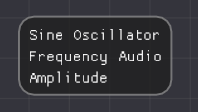
\includegraphics[width=0.5\linewidth]{graphics/sineoscillatornode.png}
    \caption{Sine Oscillator Node in \textit{Audio Editor} with two inputs frequency and amplitude and one output audio.}
    \label{fig:sineoscillator}
\end{figure}

The same method is used to implement other \texttt{AudioNodes} and enable the user to create their own nodes to manipulate audio.

Current collection of audio nodes categorized:
\begin{itemize}
    \item Generators
        \begin{itemize}
            \item Sine Oscillator
            \item Triangle Oscillator
            \item Sawtooth Oscillator
            \item Square Oscillator

        \end{itemize}
    \item Modifiers
        \begin{itemize}
            \item Add Signal
            \item Sub Signal
            \item Float Multiply
            \item Simple Click Filter
            \item General Click Filter
            \item Real Time General Click Filter
        \end{itemize}
    \item Input
        \begin{itemize}
            \item Read From WAV
        \end{itemize}
    \item Output
        \begin{itemize}
            \item Write To WAV
            \item Line Out
        \end{itemize}
    \item Utilities
        \begin{itemize}
            \item Float Range
            \item Value Float
        \end{itemize}        
    \item Editor
        \begin{itemize}
            \item Signal Graph
            \item File
        \end{itemize}
\end{itemize}

\subsection{Signal Graph Node}
\textit{Signal Graph Node} is a node for visualizing audio data being sent through links in real-time. It uses \textit{ImPlot}~\cite{implot} to plot the graph of samples. Example is on figure~\ref{fig:signalgraphnode}.

\subsection{Click filter}
We tried implementing two sorts of \textit{click filters} in \texttt{AudioEngine}. A click is an artifact in sound, which we generally want to avoid. Click filters in general try to detect clicks by analyzing samples and then correct or minimize those clicks. There are two methods, which we'll call \textit{simple} and \textit{general}.

The \textit{simple} method compares two neighboring amplitudes and checks for the difference between those values. If the difference is higher than the constant threshold, those amplitudes are set to 0. This approach works fine but has its flaws, and the clicks can still be noticed, as shown in figure \ref{fig:simpleclicks}.

The \textit{general} method, however, propagates two windows through all the samples, one large window and one small window. Then it checks for the difference between the average amplitude of the samples in the small and the large window. This requires processing of data before playing it, which is not suitable for real-time audio processing, done in \textit{Audio Graph}. Because of this, we implement two different nodes:
\begin{itemize}
    \item General Click Filter
    \item Real Time General Click Filter
\end{itemize}
The \textit{General Click Filter} uses the method mentioned before, but that doesn't work in real-time, and when the user plays the audio, the program will process the data and then, after the process, output it. The \textit{Real Time General Click Filter}, however, does the data processing on chunks retrieved from the \textit{Read From WAV} node. This allows us to do real-time processing and playing of the data but produces different results. This node is shown on figure~\ref{fig:generalclickfilter}.

\section{Results}
The project resulted in a tool for curious people learning about computer sound synthesis. \textit{Audio Graph} allows users to create graphs that synthesize data without requiring prior knowledge on the subject and programming skills. The users can start using \textit{Audio Graph} out of the box and try to create a desired sound. It allows for real-time modifications to the synthesis graph while the audio is playing, resulting in better visualization of the process of synthesis and improved tunability. This overall significantly lowers the barrier to entry into computer sound production and can help understand basic concepts. The \textit{Signal Graph Node} allows for on-the-fly viewing of data while it's being processed. For example, figure~\ref{fig:simpleclicks} showcases the same signal while it's being processed before and after entering the \textit{Simple Click Filter}. \textit{Audio Graph} can also be useful to more advanced users, as its API enables programmers and sound engineers to implement and add custom nodes to the \textit{Audio Editor} and see how they manipulate the data.

\begin{figure*}[btp]
    \centering
    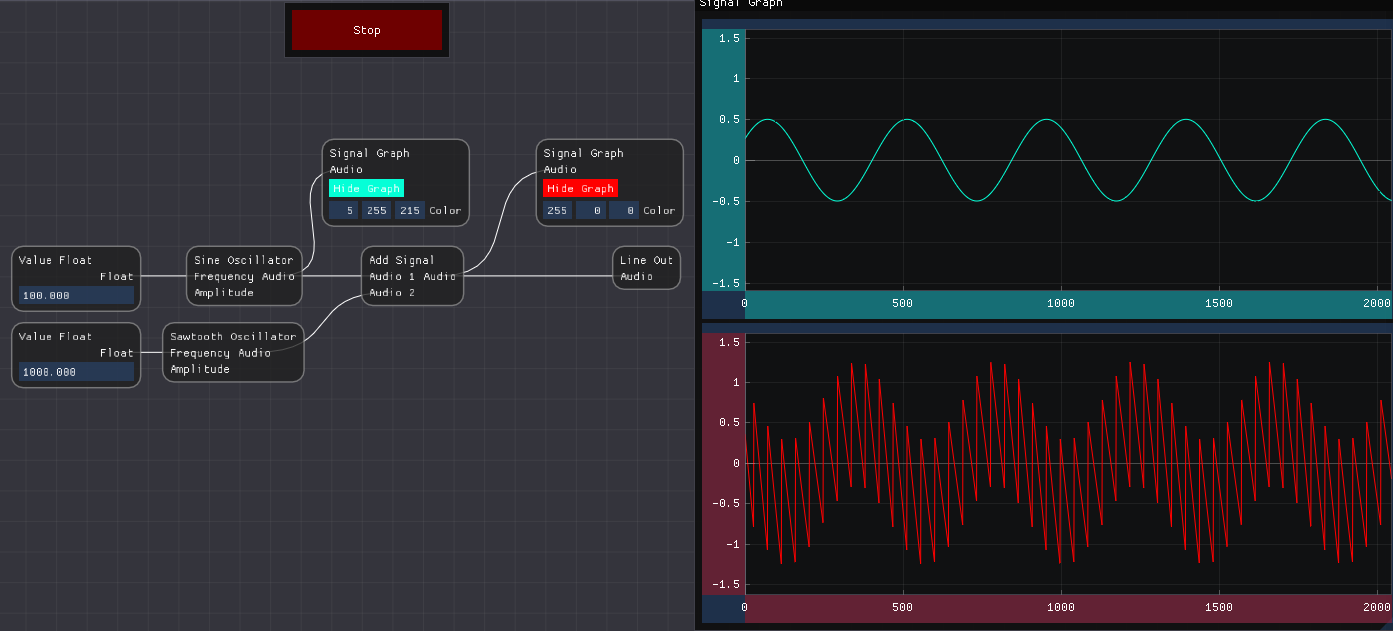
\includegraphics[width=0.85\linewidth]{graphics/signalgraphnode.png}
    \caption{A sine oscillator signal and a sawtooth oscillator signal added together with intermediate signal graphs. The blue graph represents the raw sine wave from the Sine Oscillator while the red showcases the two signals summed together. The click position is marked with red.}
    \label{fig:signalgraphnode}
\end{figure*}

\begin{figure*}[btp]
    \centering
    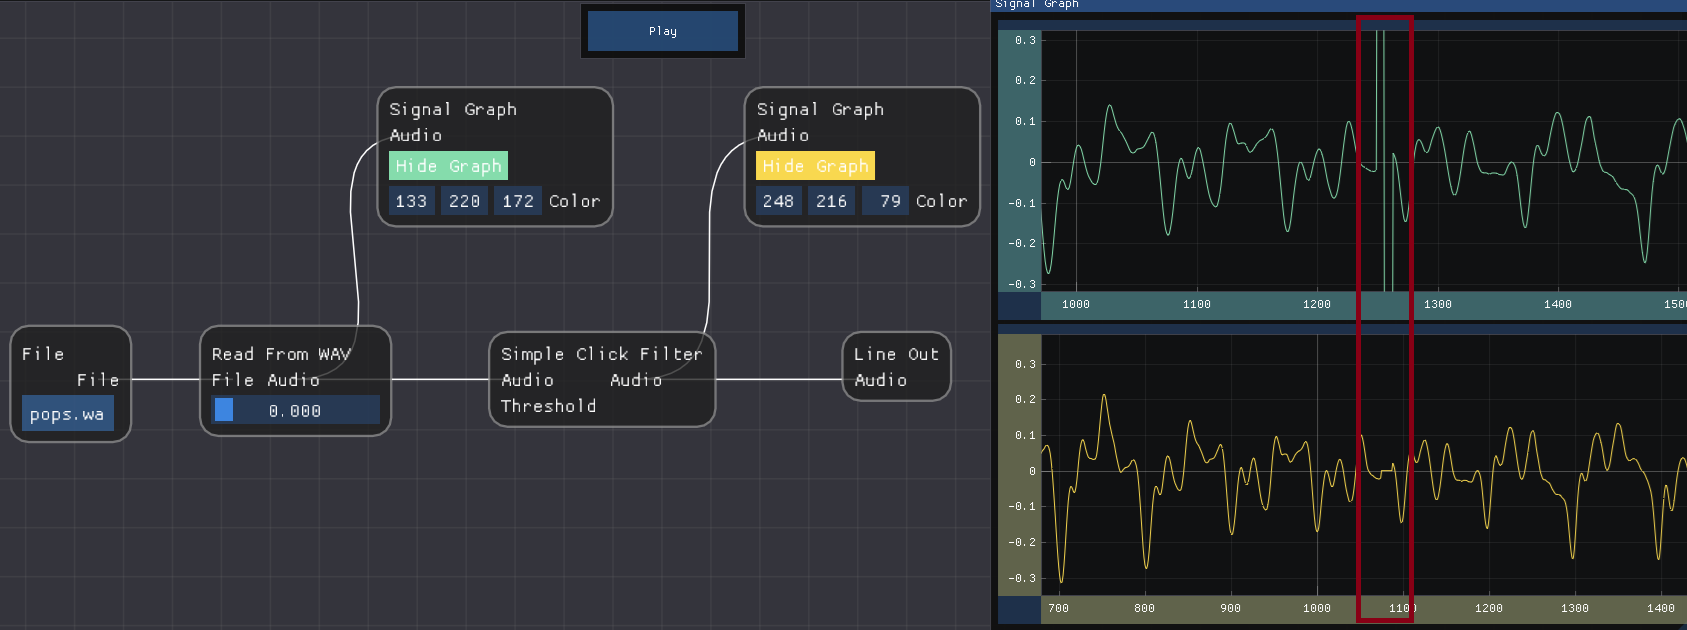
\includegraphics[width=0.9\linewidth]{graphics/simpleclickfilter.png}
    \caption{Graph of a simple click filter on a wav file. Top, blue graph, shows the signal before the click is removed while the second, yellow graph, shows the click being flattened to 0.}
    \label{fig:simpleclicks}
\end{figure*}

\begin{figure*}[btp]
    \centering
    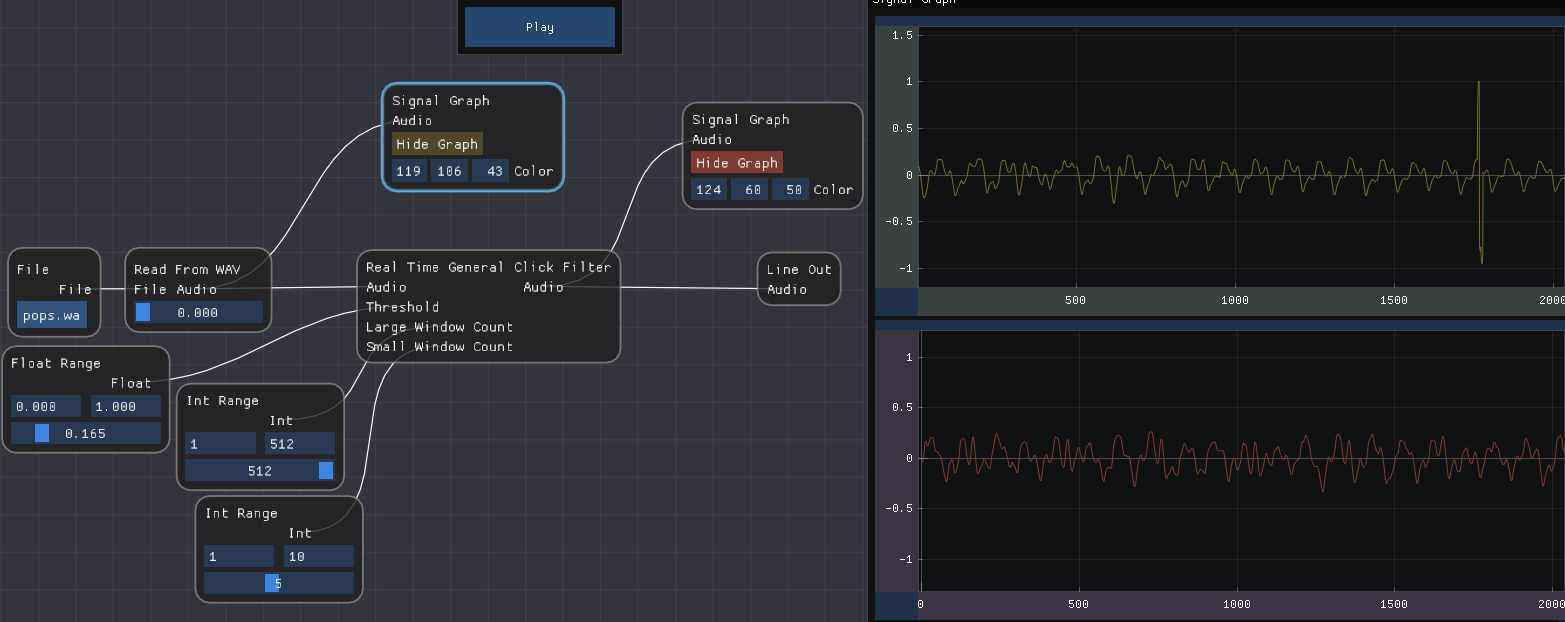
\includegraphics[width=0.9\linewidth]{graphics/generalclickfilter.png}
    \caption{Graph of a general click filter on a wav file. Top, yellow graph, shows the original signal before the click is removed while the second, red graph, shows the signal being modified with interpolation to remove the click.}
    \label{fig:generalclickfilter}
\end{figure*}

\section{Conclusion}
The project addresses the high barrier to entry of computer sound production. A lot of tools on the market currently either require prior knowledge on the subject and programming skills or are offered as a complete package without much customizability and insight into the implementation. We implemented an application that allows users to create new synthesis graphs from scratch just by "playing with" the nodes provided and instantly hear the result of that graph. It allows for on-the-fly viewing of the data while it's being processed. On the other hand, the tool allows for the creation of custom nodes and insight into the implementation of said nodes. The paper showcases and explains a few examples of graphs and nodes assembled with \textit{Audio Graph} and presents the data while it's being modified by nodes. Another aspect of the tool is that it enables simple implementation of new nodes for audio manipulation and can grow and update with time.

\begin{thebibliography}{1}
\bibitem{jsyn}
JSyn:~API for developing interactive sound applications in Java https://www.softsynth.com/jsyn/

\bibitem{audionodes}
Audio Nodes https://www.audionodes.com/

\bibitem{opengl}
OpenGL https://www.opengl.org/

\bibitem{glad}
Glad https://github.com/Dav1dde/glad

\bibitem{glfw}
GLFW https://www.glfw.org/

\bibitem{imgui}
ImGui:~API for GUI in C++ https://github.com/ocornut/imgui

\bibitem{imguinodeeditor}
Imgui Node Editor:~Implementation of a node editor using ImGui https://github.com/thedmd/imgui-node-editor

\bibitem{implot}
ImPlot:~Implementation for creating interactive plots https://github.com/epezent/implot

\bibitem{imguifiledialog}
ImGuiFileDialog:~Implementation of a file selection dialog using ImGui https://github.com/aiekick/ImGuiFileDialog

\bibitem{rtaudio}
RtAudio:~API for realtime audio input/output in C++ https://github.com/thestk/rtaudio

\bibitem{audiofile}
AudioFile:~A simple header-only C++ library for reading and writing audio files https://github.com/adamstark/AudioFile

\end{thebibliography}

\end{document}
